\documentclass[11pt]{article}
\usepackage[margin=0.8in]{geometry}
\usepackage[T1]{fontenc}
\usepackage{lmodern}
\usepackage{graphicx}
\usepackage{booktabs}
\usepackage{xcolor}
\usepackage{listings}
\usepackage{hyperref}
\usepackage{float}
\definecolor{codebg}{HTML}{F6F8FA}
\definecolor{codekw}{HTML}{2457A6}
\definecolor{codestr}{HTML}{A31515}
\definecolor{codecom}{HTML}{547547}
\lstset{language=Python,basicstyle=\ttfamily\small,backgroundcolor=\color{codebg},
 keywordstyle=\color{codekw}\bfseries,stringstyle=\color{codestr},
 commentstyle=\color{codecom}\itshape,showstringspaces=false,breaklines=true,
 frame=single,rulecolor=\color{black!18},columns=fullflexible}
\title{eBay-style Proxy Bidding with No Reserve Price}
\author{EDSL shared-state experiment setup}
\date{\today}
\begin{document}
\maketitle
\begin{abstract}
This standalone document specifies the shared-state implementation and planned
execution for this archived llm-auction condition. It does not report model
outcome estimates; any prior partial execution is identified below.
\end{abstract}
\section{Condition and protocol}
eBay-style Proxy Bidding with No Reserve Price. This condition uses
3 bidders, private values, and
100 configured auction repetitions with model gpt-4
at temperature 0.5. Each auction has 10 periods, with bidders acting serially within each period. An interview reads the current public price and the acting bidder's own maximum before its action is committed.

\begin{table}[H]\centering\begin{tabular}{ll}\toprule
Item & Setup \\\midrule
Condition & ebay\_reserve\_0 \\
Bidders & 3 \\
Value model & private \\
Configured repetitions & 100 \\
Model & gpt-4 \\
Temperature & 0.5 \\
Inference status & Prior 100-auction run interrupted after 32 completed scopes; partial state not analyzed \\
Machine & Defined; diagram generated from EDSL Machine.show\_diagram() \\
\\bottomrule\end{tabular}\caption{Experiment setup; no inference results are included.}\end{table}

\section{Shared-state machine}
Each repetition has its own scope in the shared-state map. The machine definition
is $M=(C,X,A,V,\delta,\kappa)$: constants $C$, internal state $X$, action
interface $A$, public view $V$, action transition $\delta$, and close transition
$\kappa$. Separate scopes ensure that a transition in auction $r$ cannot alter
auction $r'$. The state contains maxima $m_i$, private values $v_i$, public actions, period $t$, and current price $p$. A submitted amount $a_i$ updates $m_i\gets\max(m_i,a_i)$. With increment $\Delta$, the price is $\min(m_{(1)},m_{(2)}+\Delta)$ when the second maximum is positive, and the start price otherwise. At close, the top maximum wins if the final price meets the reserve.
\begin{figure}[H]\centering
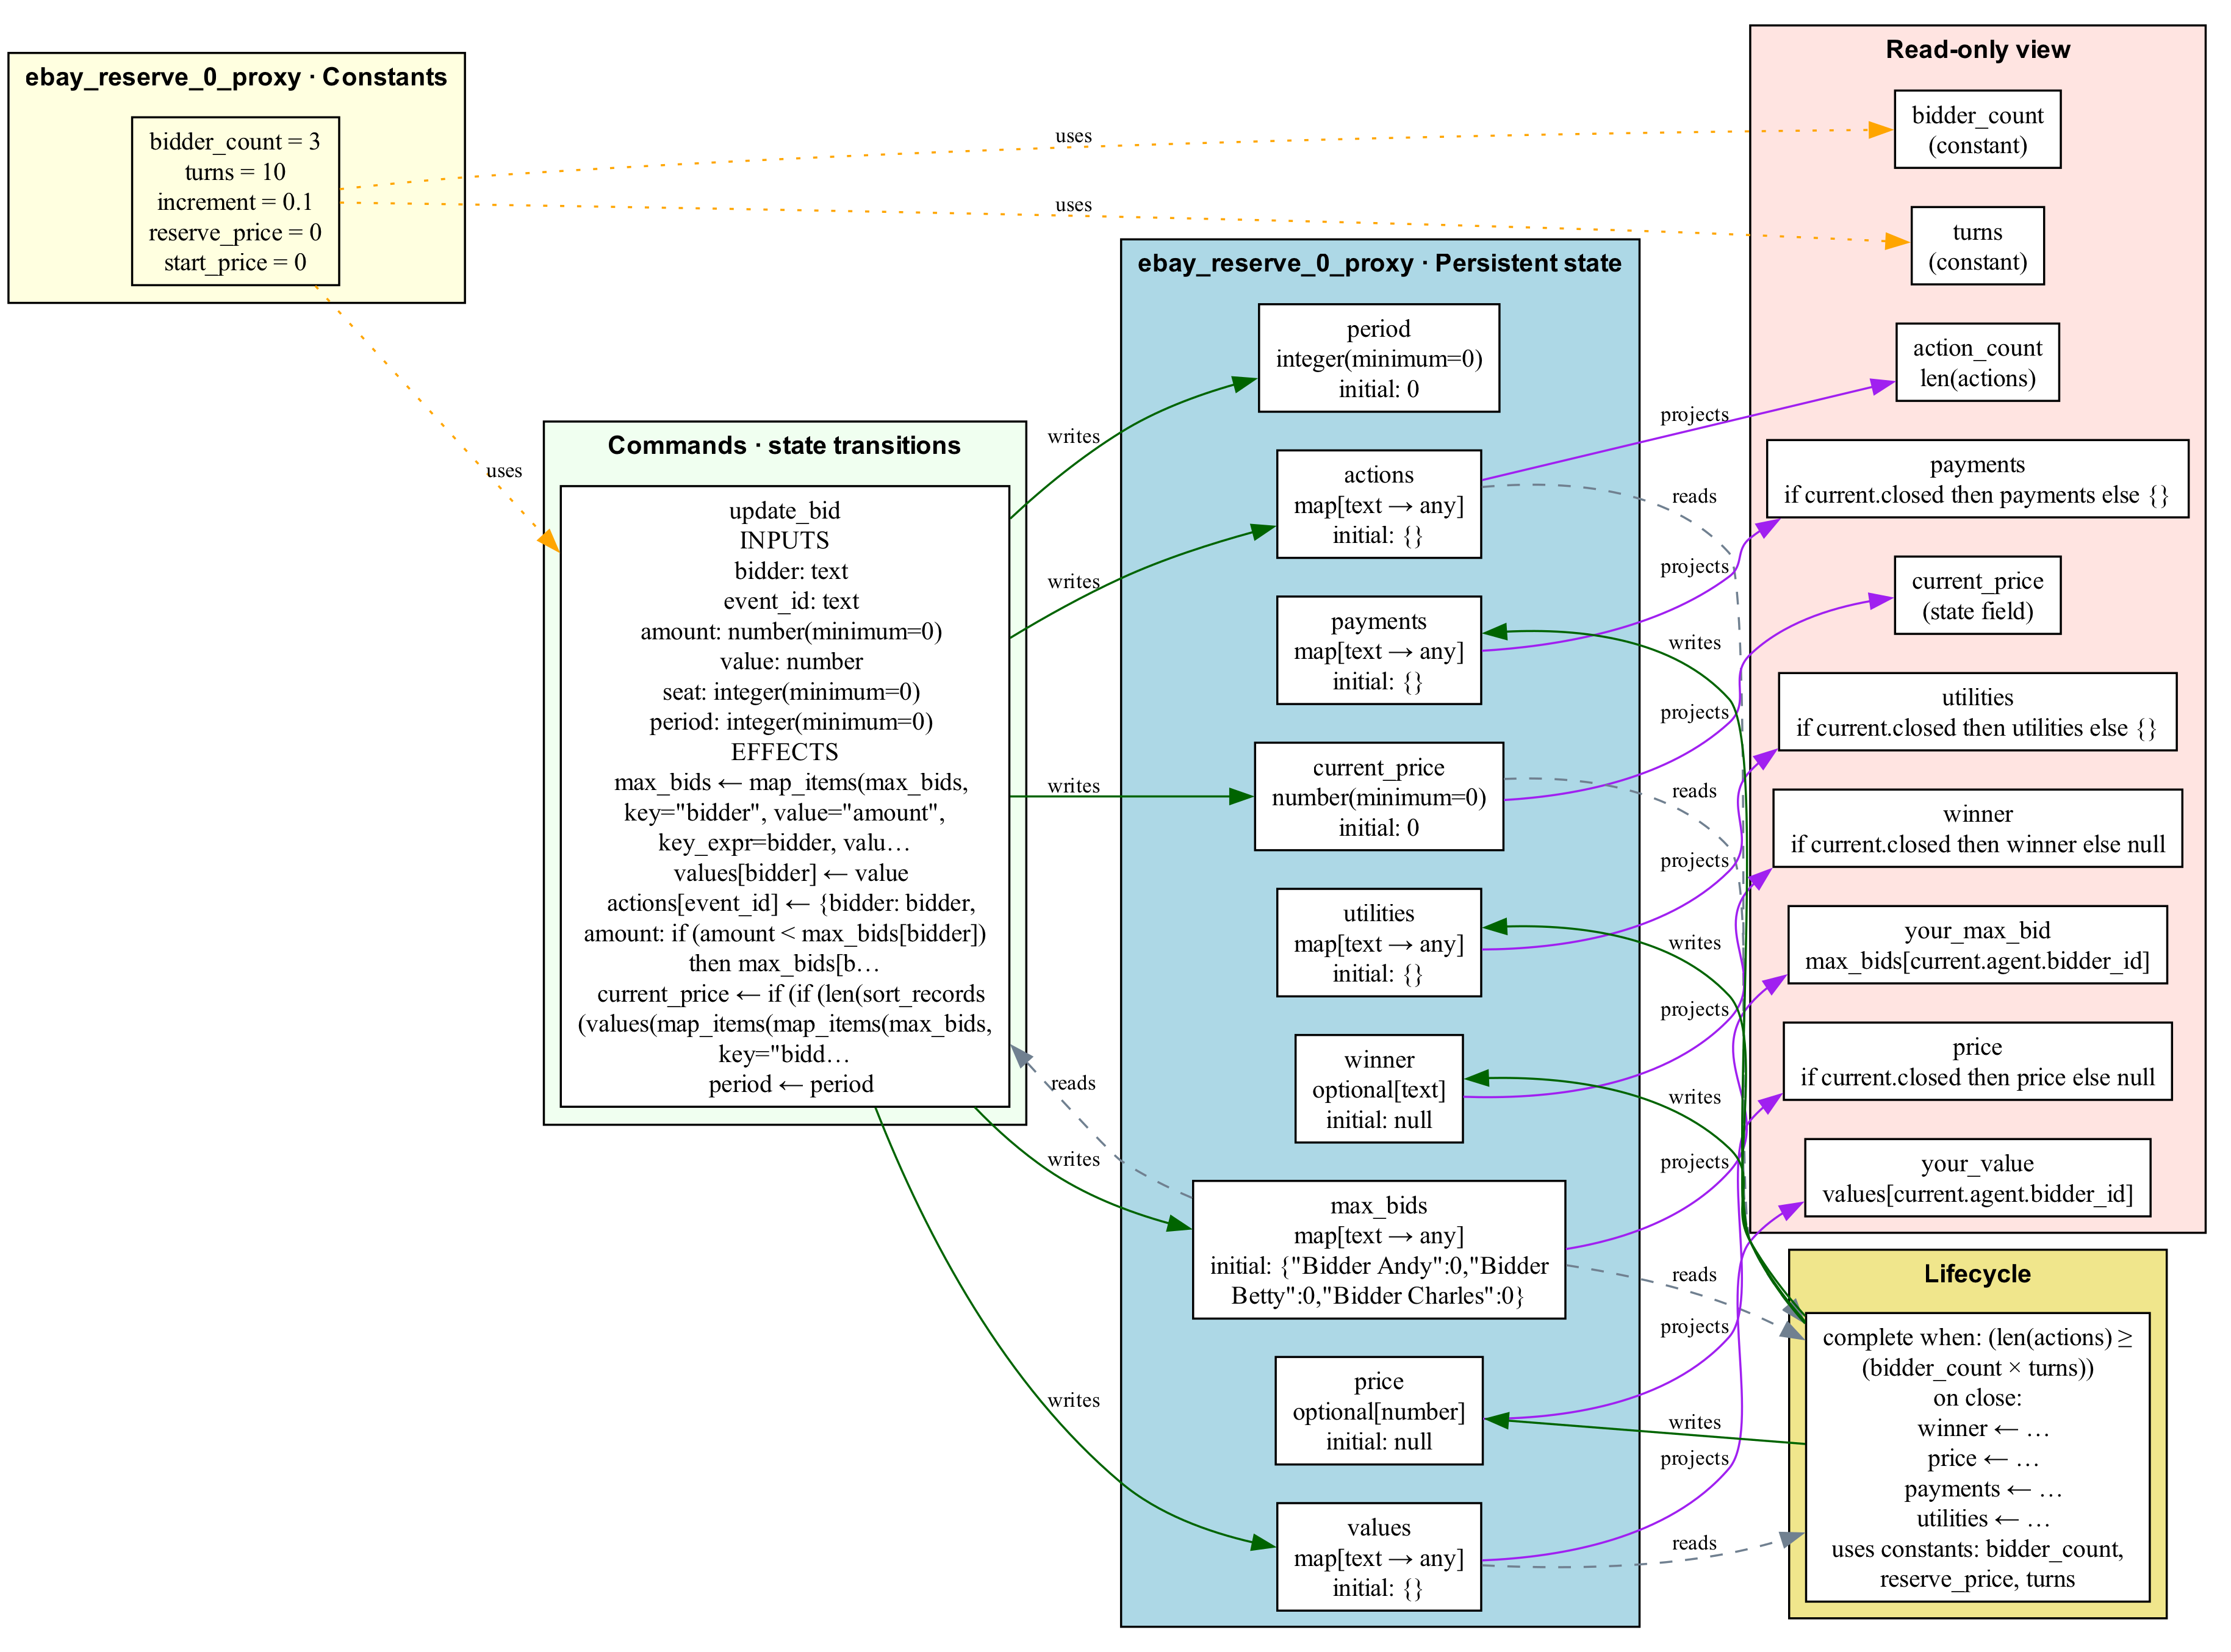
\includegraphics[width=\linewidth]{figures/state_machine.png}
\caption{Diagram generated by EDSL's \texttt{Machine.show\_diagram()}.}
\end{figure}
\subsection{Python machine factory}
The following is the implementation used to build this condition's machine.
\lstinputlisting{machine_definition.py}

\section{Launch command}
The EDSL runner executes locally and uses the model service and key configured
for this experiment. This setup step did not launch interviews. To run the
configured number of repetitions:
\begin{lstlisting}[language=bash]
python -m edsl_replication.shared_state_auctions \\
  configs/experiments/02\_01\_ebay\_reserve\_0.yaml \\
  --output edsl_replication/studies/ebay\_reserve\_0/raw_results.json
\end{lstlisting}
\section{Results}
A prior run was interrupted after 32 of 100 auction scopes completed. The completed-scope state log is preserved, but it has not been incorporated into this setup paper. No outcome estimates are reported here.
\end{document}
